\documentclass{article}
\usepackage{graphicx}

\graphicspath{ {./images/} }

\begin{document}

\section{Introduction}
This report covers the work done in modeling the phenomenon of leapfrogging vortex rings. This takes place when a vortex ring is close enough to another so that they affect the velocity and path of one another. Under the right circumstances, the two vortex rings can leapfrog one another, with one vortex ring being pulled through the other and then continuing, and then repeating the process. Using the equations that have been derived to calculate induced velocity due to a vortex, I was able to write a program that models the leapfrogging vortex rings phenomenon. 

\section{Methodology}
The equation for the induced velocity due to a vortex is

\begin{center}
\includegraphics{equation}
\end{center}

Knowing that I was going to be working with vectors and that r2 was part of the equation, I created a function that took a vector as a parameter and returned the magnitude of the vector. To continue, the 2 ring vortexes had to be seen as 4 separate vortexes (thinking of the 2 ring vortexes in a 2-d plane).

\begin{center}
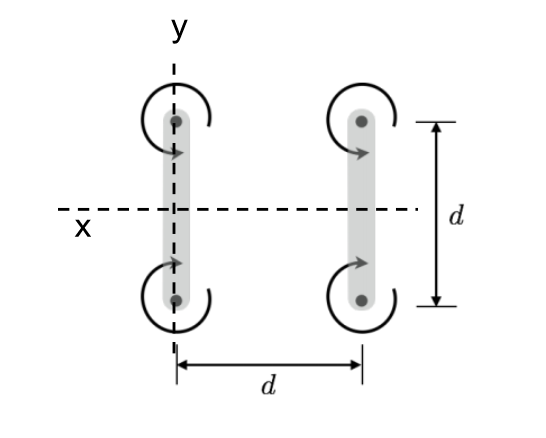
\includegraphics{vortexes}
\end{center}

I then created a function to calculate induced velocity using the above equation. It took in the position of the vortex that the induced velocity is being calculated for, the strength of the vortexes ( ), and the positions of the other three vortexes. Using these parameters, I calculated the induced velocity on the vortex in question from the three other vortexes. I then added those three induced velocities together to get the total induced velocity on the vortex in question. It is important to note that if the vortex was below the x-axis, the induced velocity had to be multiplied by -1 to be accurate, since they were rotating in the opposite direction as the others. Continuing, the total induced velocity could then be multiplied by a small time interval (in this case 0.01 seconds) to approximate the position of the vortex after that time. So, after calculating the position of each vortex after the small time interval, the whole process was repeated with the new positions of the 4 vortexes. All of the position data was then used to plot the path of the vortexes, which shows the leapfrogging ring vortexes. 

\section{Results}
The results of the program I wrote is a plot of the paths of the 4 vortexes, which shows how the leapfrogging ring vortexes look. This is that plot.

\begin{center}
\includegraphics[scale=0.62]{paths}
\end{center}

\end{document}
